\documentclass[a4paper,12pt]{article}
\usepackage[utf8]{inputenc}
\usepackage[T2A]{fontenc}
\usepackage[english, russian]{babel}
\usepackage{amsthm}
\usepackage{amsmath}
\usepackage{amssymb}
\usepackage{tikz}
\usepackage{textcomp}
\usepackage{esint}
\usepackage[unicode]{hyperref}
\usepackage{indentfirst}
\usepackage{algorithm}
\usepackage[noend]{algpseudocode}
\usepackage{amsmath,amsfonts,amssymb,amsthm,mathtools}
\usetikzlibrary{positioning,arrows}
\usepackage{graphicx}
\setlength{\topmargin}{-0.5in}
\setlength{\textheight}{9.1in}
\setlength{\oddsidemargin}{-0.4in}
\setlength{\evensidemargin}{-0.4in}
\setlength{\textwidth}{7in}
\setlength{\parindent}{0ex}
\setlength{\parskip}{1ex}
\usepackage{siunitx}

\usepackage{multicol}
\usetikzlibrary{trees}
\usepackage{fancyhdr}
\usepackage{gensymb}

\newcommand{\bbR}{\mathbb R}
\newcommand{\eps}{\varepsilon}
\newcommand{\bbN}{\mathbb N}
\newcommand{\dif}{\mathrm{d}}

\pagestyle{fancy}
\makeatletter
\fancyhead[L]{}

\fancyfoot[R]{\thepage}
\fancyfoot[C]{}

\renewcommand{\maketitle}{
	\noindent{\bfseries\scshape\large\@title\ \mdseries\upshape}\par
	\noindent {\large\itshape\@author}
	\vskip 2ex}
\makeatother




\begin{document}
	
\Large \textbf { \begin{center}
		Работа 1.3\\ Эффект Рамзауэра \\
		Селюгин Михаил, 876 \\
\end{center}}


	\section{Теория вопроса}
	
	Эффективное сечение реакции --- это величина, характеризующая вероятность перехода системы двух сталкивающихся частиц в результате их рассеяния (упругого или неупругого) в определенное конечное состояние. Сечение $\sigma$ это отношение числа таких переходов $N$ в единицу времени к плотности потока $nv$ рассеиваемых частиц, падающих на мишень, т.е. к числу частиц, попадающих в единицу времени на единичную площадку, перпендикулярную к их скорости.
	
	\begin{equation}
	\sigma = \frac{N}{nv}
	\end{equation}
	
	Для изучения зависимости сечения электронов от падающей энергии Рамзауэр провел серию опытов, где пучок электронов, вылетая с катода К, проходит ускоряющую разность потенциалов $V$, приложенную между катодом и электродом Э. Часть электронов рассеивается на атомах и собирается коллектором КЛ, оставшиеся же долетают до анода А и формируют анодный ток.
	
	
	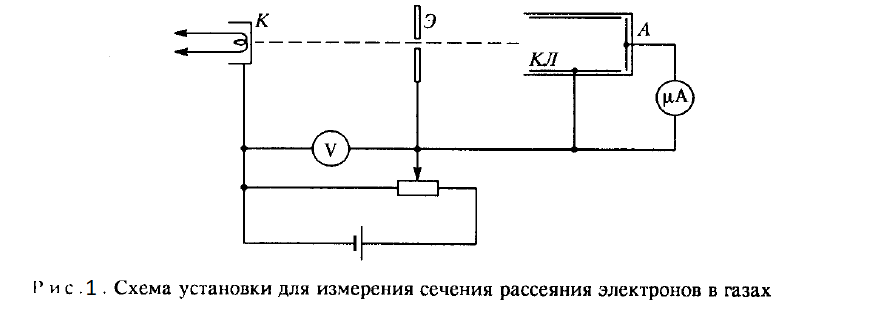
\includegraphics[height= 10\baselineskip]{scheme.png}
	
	
	Классическая теория предсказывала уменьшение сечения с ростом напряжения $V$, однако в ходе опытов была получена иная принципиальная зависимость, получившая название эффект Рамзауэра.
	
	\begin{center}
		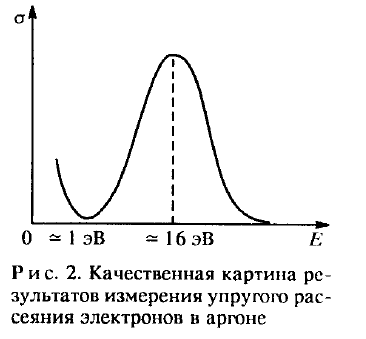
\includegraphics[]{princip.png}
	\end{center}
	
	
	Эффект Рамзауэра нельзя объяснить с позиций классической теории. С квантовой же точки зрения картина рассеяния выглядит следующим образом. Внутри атома потенциальная энергия налетающего электрона отлична от нуля, скорость электрона меняется, становясь равной $v'$ в соответсвии с законом сохранения энергии:
	\begin{equation}
	E = \frac{mv^2}{2} = \frac{mv'^2}{2} + U
	\end{equation}
	
	а значит, изменяется и длина его волны де Бройля. Таким образом, по отношению к электронной волне атом ведет себя как преломляющая среда с относительным показателем преломления:
	
	\begin{equation}
	n = \frac{\lambda}{\lambda'} = \sqrt{1 - \frac{U}{E}}
	\end{equation}
	
	Решение задачи о рассеянии электрона на сферическом потенциале достаточно громоздко. Поэтому рассмотрим более простое одномерное приближение: электрон рассеивается на потенциальной яме конечной глубины. Уравнение Шрёдингера в этом случае имеет вид:
	\begin{equation}
	\psi'' + k^2\psi = 0 \qquad k^2 = \begin{cases}
	k_1^2  = \frac{2mE}{\hbar^2} \\
	k_2 = \frac{2m(E+U_0)}{\hbar^2}
	\end{cases}
	\end{equation}
	
	Коэффициент прохождения равен отношению квадратов амплитуд прошедшей и падающей волн и определяется выражением:
	\begin{equation}
	D = \frac{16k_1^2k_2^2}{16k_1^2k_2^2 + 4(k_1^2-k_2^2)^2\sin^2(k_2l)}
	\end{equation}
	
	Видно, что коэффициент прохождения частицы над ямой, в зависимости от её энергии, имеет вид чередующихся максимумов и минимумов. В частности, если $k_2l = \pi$, то коэффициент прохождения равен 1, т.е. отраженная волна отсутствует, и электрон беспрепятственно проходит через атом. Этот эффект является квантовым аналогом просветления оптики. Таким образом, коэффициент прохождения электронов максимален при условии:
	\begin{equation}
	k_2l = \sqrt{\frac{2m(E+U_0)}{\hbar^2}}l = \pi n
	\end{equation}
	Прошедшая волна 1 усилится волной 2, если геометрическая разность хода между ними $\Delta = 2l = \lambda'$, что соответствует условию первого интерференционного максимума, т.е.
	\begin{equation}
	2l = \frac{h}{\sqrt{2m(E_1 + U_0)}}
	\end{equation}
	C другой стороны, прошедшая волна ослабится, если $2l = \frac{3}{2}\lambda'$, т.е.
	\begin{equation}
	2l = \frac{3}{2}\frac{h}{\sqrt{2m(E_2+U_0)}}
	\end{equation}
	Решая эти уравнения совместно можно исключить $U_0$ и найти эффективный размер атома $l$:
	\begin{equation}
	l = \frac{h\sqrt{5}}{\sqrt{2m(E_2-E_1)}}
	\end{equation}
	Понятно, что энергии $E_1$, $E_2$ соответсвуют энергия электронов, прошедших разность потенциалов $V_1$ и $V_2$.
	Кроме того, можно оценить эффективную глубину потенциальной ямы атома:
	\begin{equation}
	U_0 =\frac{4}{5}E_2 - \frac{9}{5}E_1
	\end{equation}
	
	Теперь рассмотрим ВАХ тиратрона. Она имеет вид:
	$$
	I_a = I_0e^{-C\omega(V)}, C = Ln_a\Delta_a
	$$
	где $I_0 = eN_0$ --- ток катода, $I_a = eN_a$ --- анодный ток, $\Delta_a$ --- площадь поперечного сечения атома, $n_a$ --- концентрация атомов газа в лампе, $L$ --- расстояние от катода до анода, $\omega(V)$ --- вероятность рассеяния электрона на атоме как функция от ускоряющего напряжения. По измеренной ВАХ тиратрона можно определить зависимость вероятности рассеяния электрона от его энергии из соотношения:
	\begin{equation}
	\omega(V) = -\frac{1}{C}\ln\frac{I_a}{I_0}
	\end{equation}
	
	\section{Экспериментальная установка}
	В данной работе используется тиратрон ТГ3-01/1.3Б, заполненный инертным газом.
	
	
	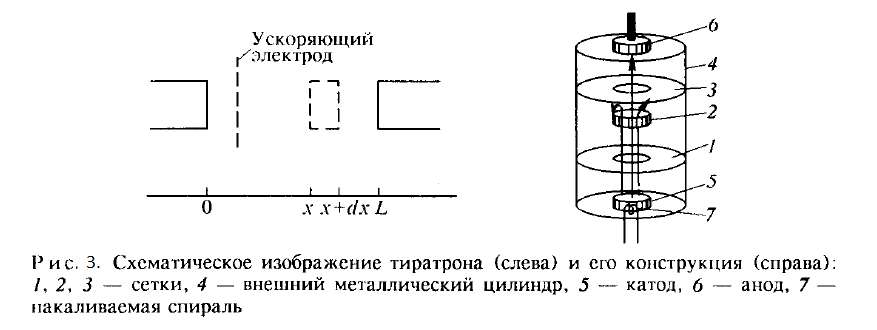
\includegraphics[height=10\baselineskip, width=\linewidth]{tira.png}
	
	Теперь рассмотрим ВАХ тиратрона. Она имеет вид:
	$$
	I_a = I_0e^{-C\omega(V)}, C = Ln_a\Delta_a
	$$
	где $I_0 = eN_0$ --- ток катода, $I_a = eN_a$ --- анодный ток, $\Delta_a$ --- площадь поперечного сечения атома, $n_a$ --- концентрация атомов газа в лампе, $L$ --- расстояние от катода до анода, $\omega(V)$ --- вероятность рассеяния электрона на атоме как функция от ускоряющего напряжения. 
	\newpage
	
	 По измеренной ВАХ тиратрона можно определить зависимость вероятности рассеяния электрона от его энергии из соотношения:
	\begin{equation}
	\omega(V) = -\frac{1}{C}\ln\frac{I_a}{I_0}
	\end{equation}
	
	\section{Результаты измерений и вычислений}
	\subsection{Динамический режим}
	{\bf 1.} На экране осциллографа была получена ВАХ тиратрона для двух значений напряжения лампы накала:
	$$V_1 = 2,81B\ V_2 = 3,08B$$
	
\begin{center}
	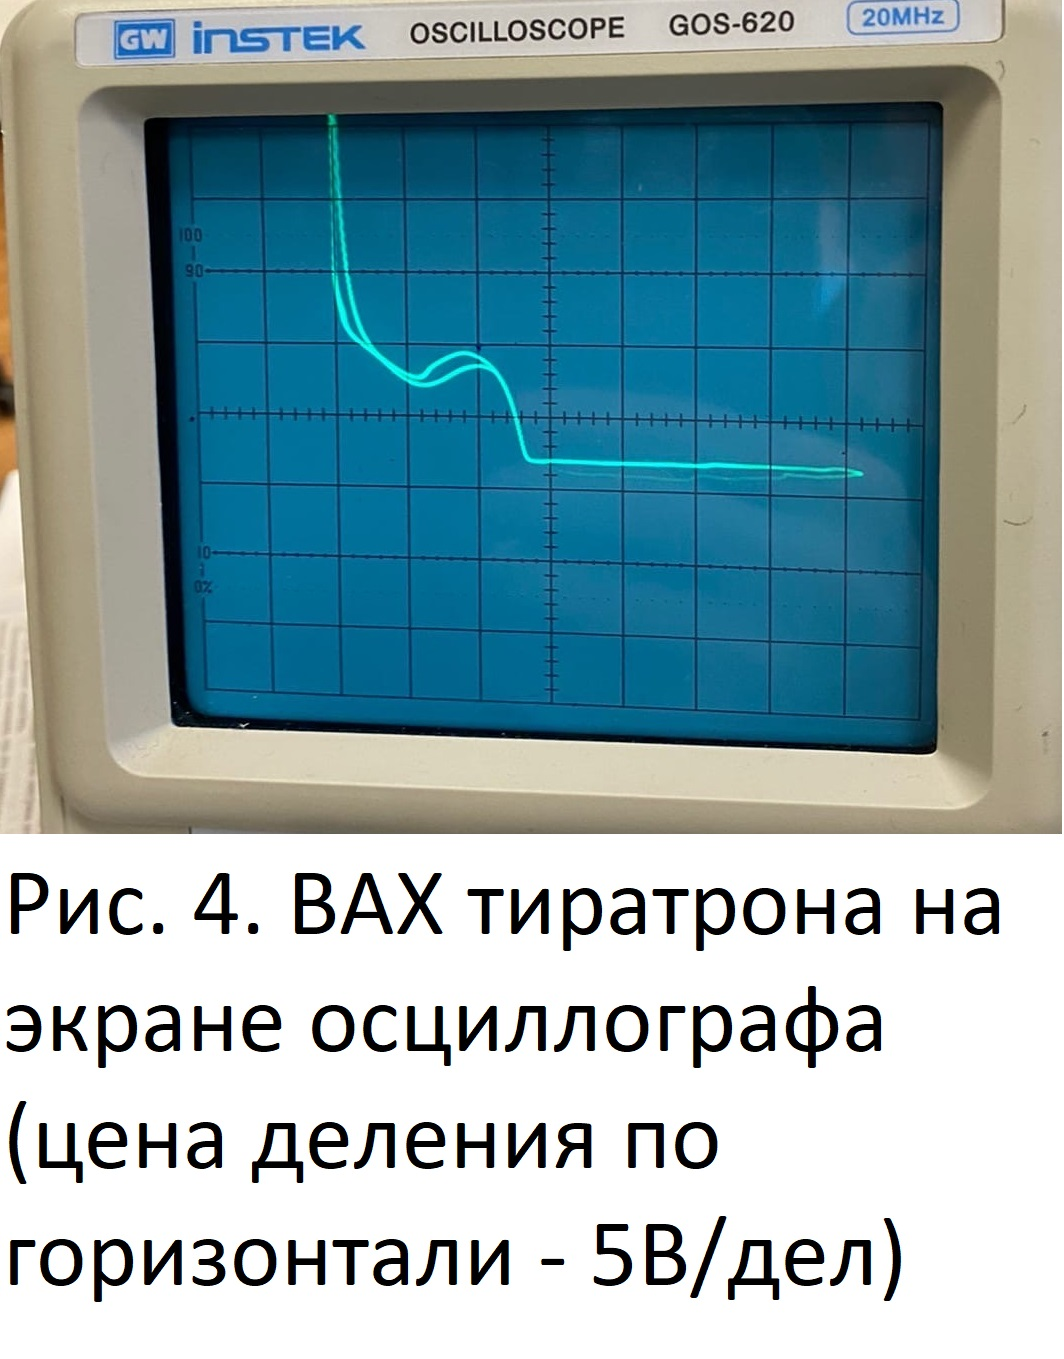
\includegraphics[height=13\baselineskip]{vakh.jpg}
\end{center}	
	
\newpage	{\bf 2.} По полученным кривым определим абсциссы первых максимума и минимума функции $I_a(V),$ а также значения напряжения пробоя $V_{\text{проб}}$
	
	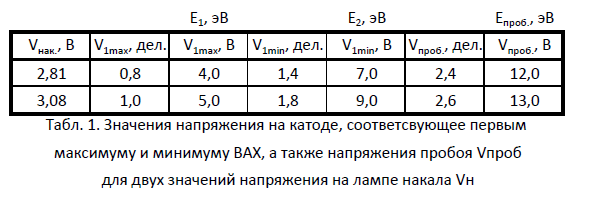
\includegraphics[width=\linewidth]{tabl1.png}
	
	{\bf 3.} Воспользуемся формулами $(9), (10)$ и вычислим размер атома $l$ и глубину потенциальной ямы $U_0$.
	$U = 2,81B:$
	$$l \approx 0,34A, \ U_0 \approx 1,6\text{эВ}$$
	$U = 3,08B:$
	$$l \approx 0,38A, \ U_0 \approx 1,8\text{эВ}$$
	
	{\bf 4.} Оценим погрешность
	
	$\sigma_E = 0,05$ дел, значит $\sigma_{U_0} =\sqrt{0,2^2+0,35^2}= 0,4$В
	
	$$\sigma_{E_2 - E_1} = \sqrt{2\cdot 0,05^2} \approx 0,07\text{дел.}$$ 
	
	$$\eps_{E_2 - E_1} = \frac{0,07}{0,7} = 0,1 \Rightarrow \eps_l = 0,5\eps_{E_2 - E_1} = 0,05$$
	Окончательно, имеем
	$$l = 0,36 \pm0,02 A\ (\eps = 5\%)$$
	$$U_0 = 1,7 \pm 0,4 \text{эВ} \ (\eps = 24\%)$$
	
	{\bf 5.} Из полученного значения напряжения пробоя $V_{\text{проб} } = 12-13B$ сделаем вывод, что тиратрон наполнен ксеноном $(12,1B)$.
	
	\subsection{Статический режим}
	{\bf 1.} В статическом режиме измеряем зависимость напряжения на аноде от напряжения на катоде. Учитывая $R_a = 100kOm$, рассчитаем ток анода и построим ВАХ тиратрона. 
	Также с помощью $(12)$ рассчитаем значение вероятности рассеяния электрона.
	
	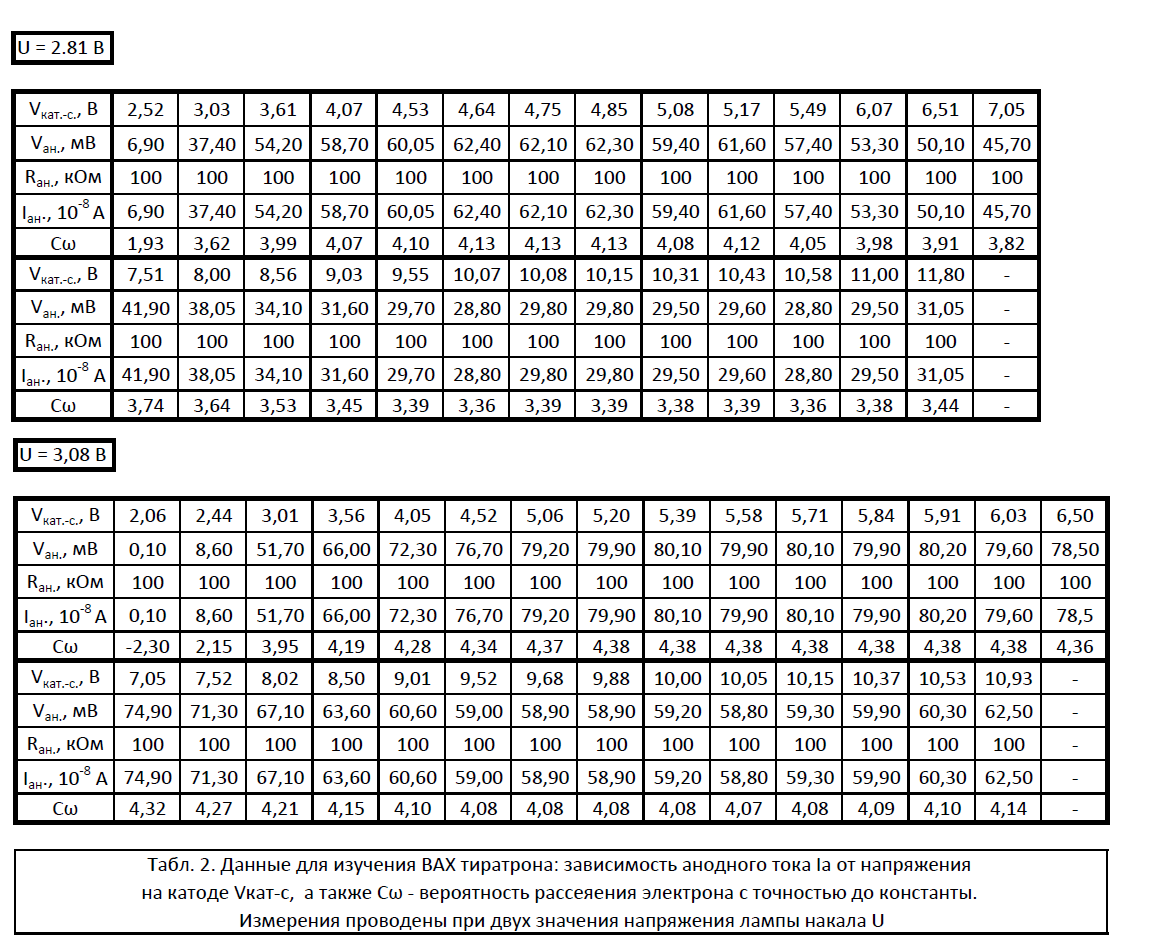
\includegraphics[width=1.1\linewidth]{tabl2.png}
	 
	 \newpage
	 
	{\bf 2.} По данным табл. 2 построим график ВАХ тиратрона и график зависимости вероятности рассеяния от напряжения на катоде.
	
	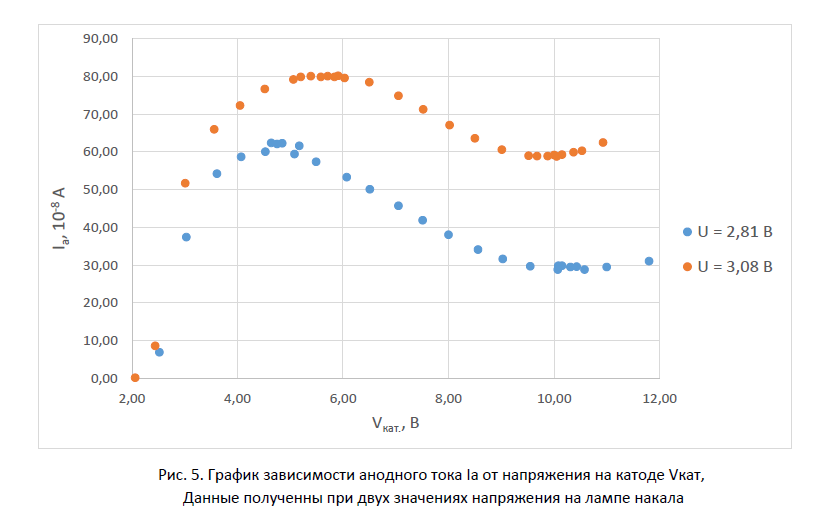
\includegraphics[width=\linewidth]{graph1.png}
	
	
	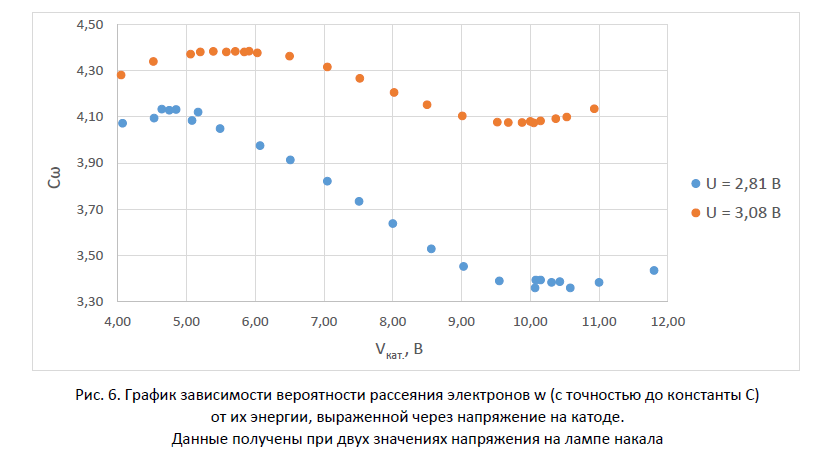
\includegraphics[width=\linewidth]{graph2.png}
	
	
	{\bf 3.} Используя формулу (6), найдем значения $E_n$, которым соответствуют максимумам на графике ВАХ:
	$$E_n = n^2(E_1+U_0)-U_0$$
	$$E_2 = 13,4 \pm 0,2 \text{эВ}$$
	$$E_3 = 32,8 \pm 0,2 \text{эВ}$$
	
	Однако данные максимумы пронаблюдать не удалось, так как при $U = 12B$ происходит пробой.
	
	Но максимумы, определенные по графику 5, совпали с максимумами, рассчитанными на экране осциллографа динамическим методом. ($U_1 \approx 4B, \ U_2 \approx 5B$)
	
	Если говорить о вероятности рассеяния, рассчитанной по формуле
	$$C\omega (I_k) = \ln\frac{I_a(I_k)}{I_0},$$ то ее график близок к предсказанному теоретически.
	
	\section{Вывод}
	В данной работе был исследован эффект Рамзауэра -- рассеяние медленных электронов на атомах.
	
	Была получена ВАХ тиратрона в статическом и динамическом режимах работы. Было выявлено, что в опыте используется ксенон, а также получена оценка эффективного размера атома и глубины потенциальной ямы. 
		$$l = 0,36 \pm0,02 A\ (\eps = 5\%)$$
	$$U_0 = 1,7 \pm 0,4 \text{эВ} \ (\eps = 24\%)$$
	
	Также была получена зависимость вероятности рассеяния электрона от его энергии и эта зависимость, качественно, оказалась близка к предсказанной теоретически.
	
	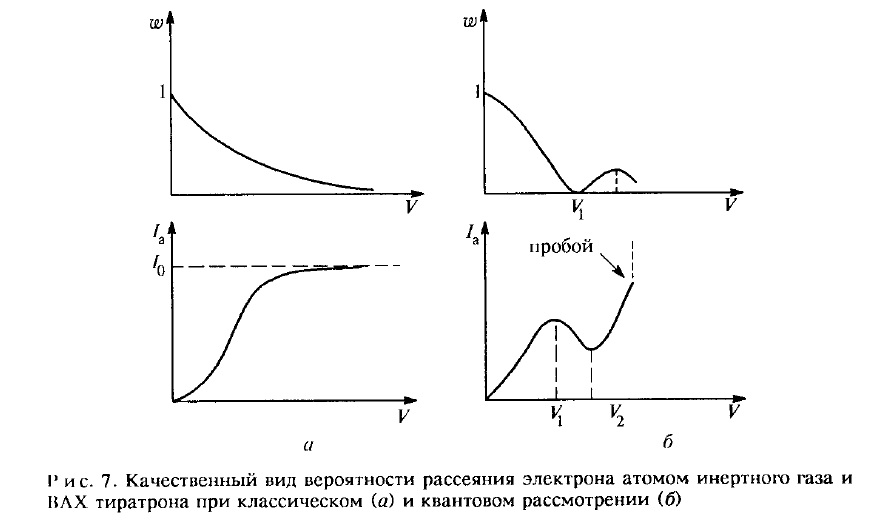
\includegraphics[width=\linewidth]{teor.png}
	
	 
\end{document}